\section{Příklad 3}
\tretiZadani{E}

\begin{enumerate}
    \item
    \textbf{Nahrazení napěťového zdroje}
    \newline
    Nejprve si nahradíme napěťový zdroj za proudový pro jednodušší počítání vodivostí do následného
    dosazení do matice. Pro náhradu napěťového zdroje platí: ${I_z} = \frac{{U}}{R_5}$
    \newline
    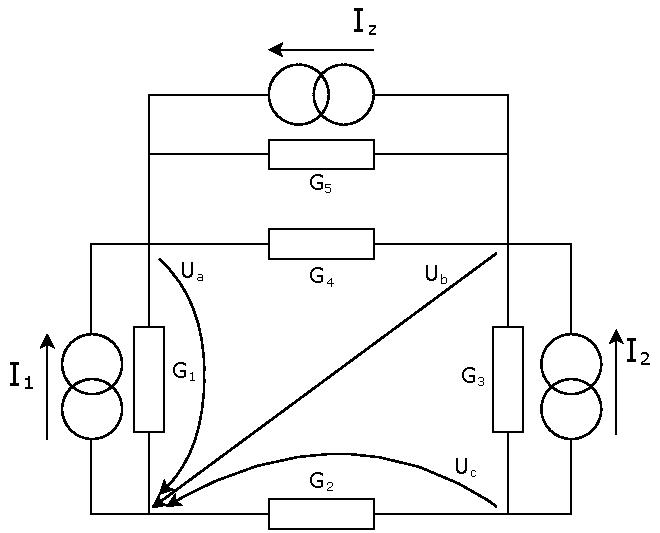
\includegraphics[scale=0.7]{pr3/pr3.pdf}
    \newline
    \item
    \textbf{Najdeme základní proud:}\\\\
    ${I_z} = \frac{{U}}{R_5} = \frac{{135 V}}{21 \Omega} = 6,4286A$
    \item
    \textbf{Sestavíme matice:}
    \newline
    $
    \begin{pmatrix}
    	G_1+G_4+G_5&-G_4-G_5&0\\
    	-G_4-G_5&G_3+G_4+G_5&-G_3\\
    	0&-G_3&G_2+G_3
    \end{pmatrix}\times 
    \begin{pmatrix}
    	U_A\\
    	U_B\\
    	U_C
    \end{pmatrix}=
    \begin{pmatrix}
    	I_z + I_1\\
    	I_2 - I_z\\
    	-I_2
    \end{pmatrix}
    $
    \\\\\\
    $
    \begin{pmatrix}
    	0,0192+0,0238+0,0476&-0,0238-0,0476&0\\
    	-0,0238-0,0476&0,0192+0,0238+0,0476&-0,0192\\
    	0&-0,0192&0,0238+0,0192
    \end{pmatrix}\times 
    \begin{pmatrix}
    	U_A\\
    	U_B\\
    	U_C
    \end{pmatrix}=
    \\\\\\
    =
    \begin{pmatrix}
    	6,4286 + 0,55\\
    	0,65 - 6,4286\\
    	-0,65
    \end{pmatrix}
    $
    \\\\\\
    $
    \begin{pmatrix}
    	6,9786\\
    	-5,7786\\
    	-0,65
    \end{pmatrix}=
    \begin{pmatrix}
    	0,0906&-0,0714&0\\
    	-0,0714&0,0906&-0,0192\\
    	0&-0,0192&0,0046
    \end{pmatrix}\times 
    \begin{pmatrix}
    	U_A\\
    	U_B\\
    	U_C
    \end{pmatrix}
    $
    \\\\\\
    $
    \begin{pmatrix}
    	6,9786\\
    	-0,2789\\
    	-0,65
    \end{pmatrix}=
    \begin{pmatrix}
    	0,0906&-0,0714&0\\
    	0&0,0343&-0,0192\\
    	0&-0,0192&0,0046
    \end{pmatrix}\times
    \begin{pmatrix}
    	U_A\\
    	U_B\\
    	U_C
    \end{pmatrix}
    $
    \\\\\\
    $
    \begin{pmatrix}
    6,9786\\
	-0,2789\\
	-0,8060
    \end{pmatrix}=
    \begin{pmatrix}
    	0,0906&-0,0714&0\\
    	0&0,0343&-0,0192\\
    	0&0&0,0061
    \end{pmatrix}\times
    \begin{pmatrix}
    	U_A\\
    	U_B\\
    	U_C
    \end{pmatrix}
    $
    \\
    \item 
    \textbf{Z matice můžeme najít $U_c$}\\\\
    $U_c * 0,0061 = -0,8060$ \\\\
    $U_c = \frac{-0,8060}{0.006`} = -132,1311$
    \item
    \textbf{Když máme $U_c$ tak najdeme $U_b$:}\\\\
    $U_b * 0.0343 - (0,0192 * (-132,1311)) =  -0,2789$\\\\
    $U_b = \frac{-0,2789 + (0,0192 * (-132,1311))}{0,0343} = 20,6282$
    \item 
    \textbf{Najdeme napětí na rezistoru $R_3$:}\\\\
    $U_{R3} = U_b - U_c$\\\\
    $U_{R3} = 20,6282 - (-132,1311) = 152,7593V$
    \item
    \textbf{Najdeme proud na rezistoru $R_3$:}
    $I_{R3} = \frac{U_{R3}}{R_3}$\\\\
    $I_{R3} = \frac{152,7593 V }{52\Omega} = 2,9377 A$ 
\end{enumerate}